\chapter{Application architecture}
\label{sec:application-architecture}
	
%	TODO: rewrite intro
    This chapter covers the application architecture. We present here the essential services and application components that enact the current and the new life-cycle processes.

	\section{Prototypical application structure}
	
	This section presents the application architecture from the solution architecture point of view. A generic solution architecture is depicted in Figure \ref{fig:application-view}.
	
	The application architecture presented covers the application as a ``white box'', its internal component structure, services and interfaces with adjacent applications. Typically the solutions architecture takes the technology aspects into account, accounting for parts of the infrastructure.
	
    \begin{figure}[h]
		\centering
		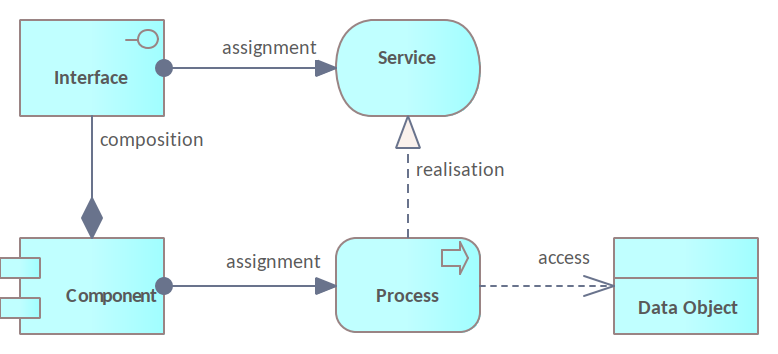
\includegraphics[width=.6\textwidth]{images/views/Application view.png}
		\caption{The prototypical application structure view}
		\label{fig:application-view}
	\end{figure}

	The central element of the application architecture is the \textit{application service}, which represents application behaviour or functionality. The application services, from an inter-layer perspective, serve the processes in the business layer and provide support for their realisation. 
	
	The application services are realised through application processes. The processes have application components assigned to them signifying their place of encapsulation. Application components are modular and replaceable blocks encapsulating implementation of application services and functionalities. In practice, for clarity, we take a shortcut, and say that the application services are realised through \textit{application components} directly.
	
	Components are said to expose interaction \textit{interfaces} which are modelled, in ArchiMate, as proper parts of the components. The interfaces are assigned to services signifying how the latter are to be accessed and consumed. 
	
	Also, components, as well as processes they encapsulate, access \textit{data objects}, which are passive components of the application architecture.

	The solution architecture presented in this section is an adaptation of the generic architecture. Here we focus on presenting what application services are used to support each business process. Moreover, we are interested in grasping the difference in the application layer, between the current and new versions of the business processes. 
	
	To do so, we split the application view diagrams into three vertical lanes. The left lane hosts the current version of the business process as well as the application services and components that are used to support it. In the right lane, we place the new business process and the new application services and components that will have to be adopted for the digital transformation. The middle lane hosts the services and components that are are currently employed and will be carried over into the new application architecture: they are common to both the current and new architectures.

	Below we present an overview of the application architecture, in terms of services alone, depicting how the asset life-cycle stages are served.	
	
	\section{LAM\#2 specific application architecture}

	This section presents the application architecture for services developed in the context of LAM\#2 project. In Section \ref{sec:application-lifecycle} these applications will be placed into the context of asset lifecycle process described in Section \ref{sec:asset-lifecycle}. 
	
	The project specific tools are \textit{the transformation tool}, \textit{the validation tool} and \textit{the online (dissemination) tool}.
	
	\subsection{LAM transformation tool}
	
	First of the three tools, is the transformation tool from structured RDF data into human readable representations. This tool contributes directly to the goal of producing and dissemination the LAM data for end-user consumption on the OP Portal. Figure \ref{fig:app-transformation-tool} depicts the application architecture, with LAM transformer component in the centre of the diagram.

    \begin{figure}[!h]
		\centering
		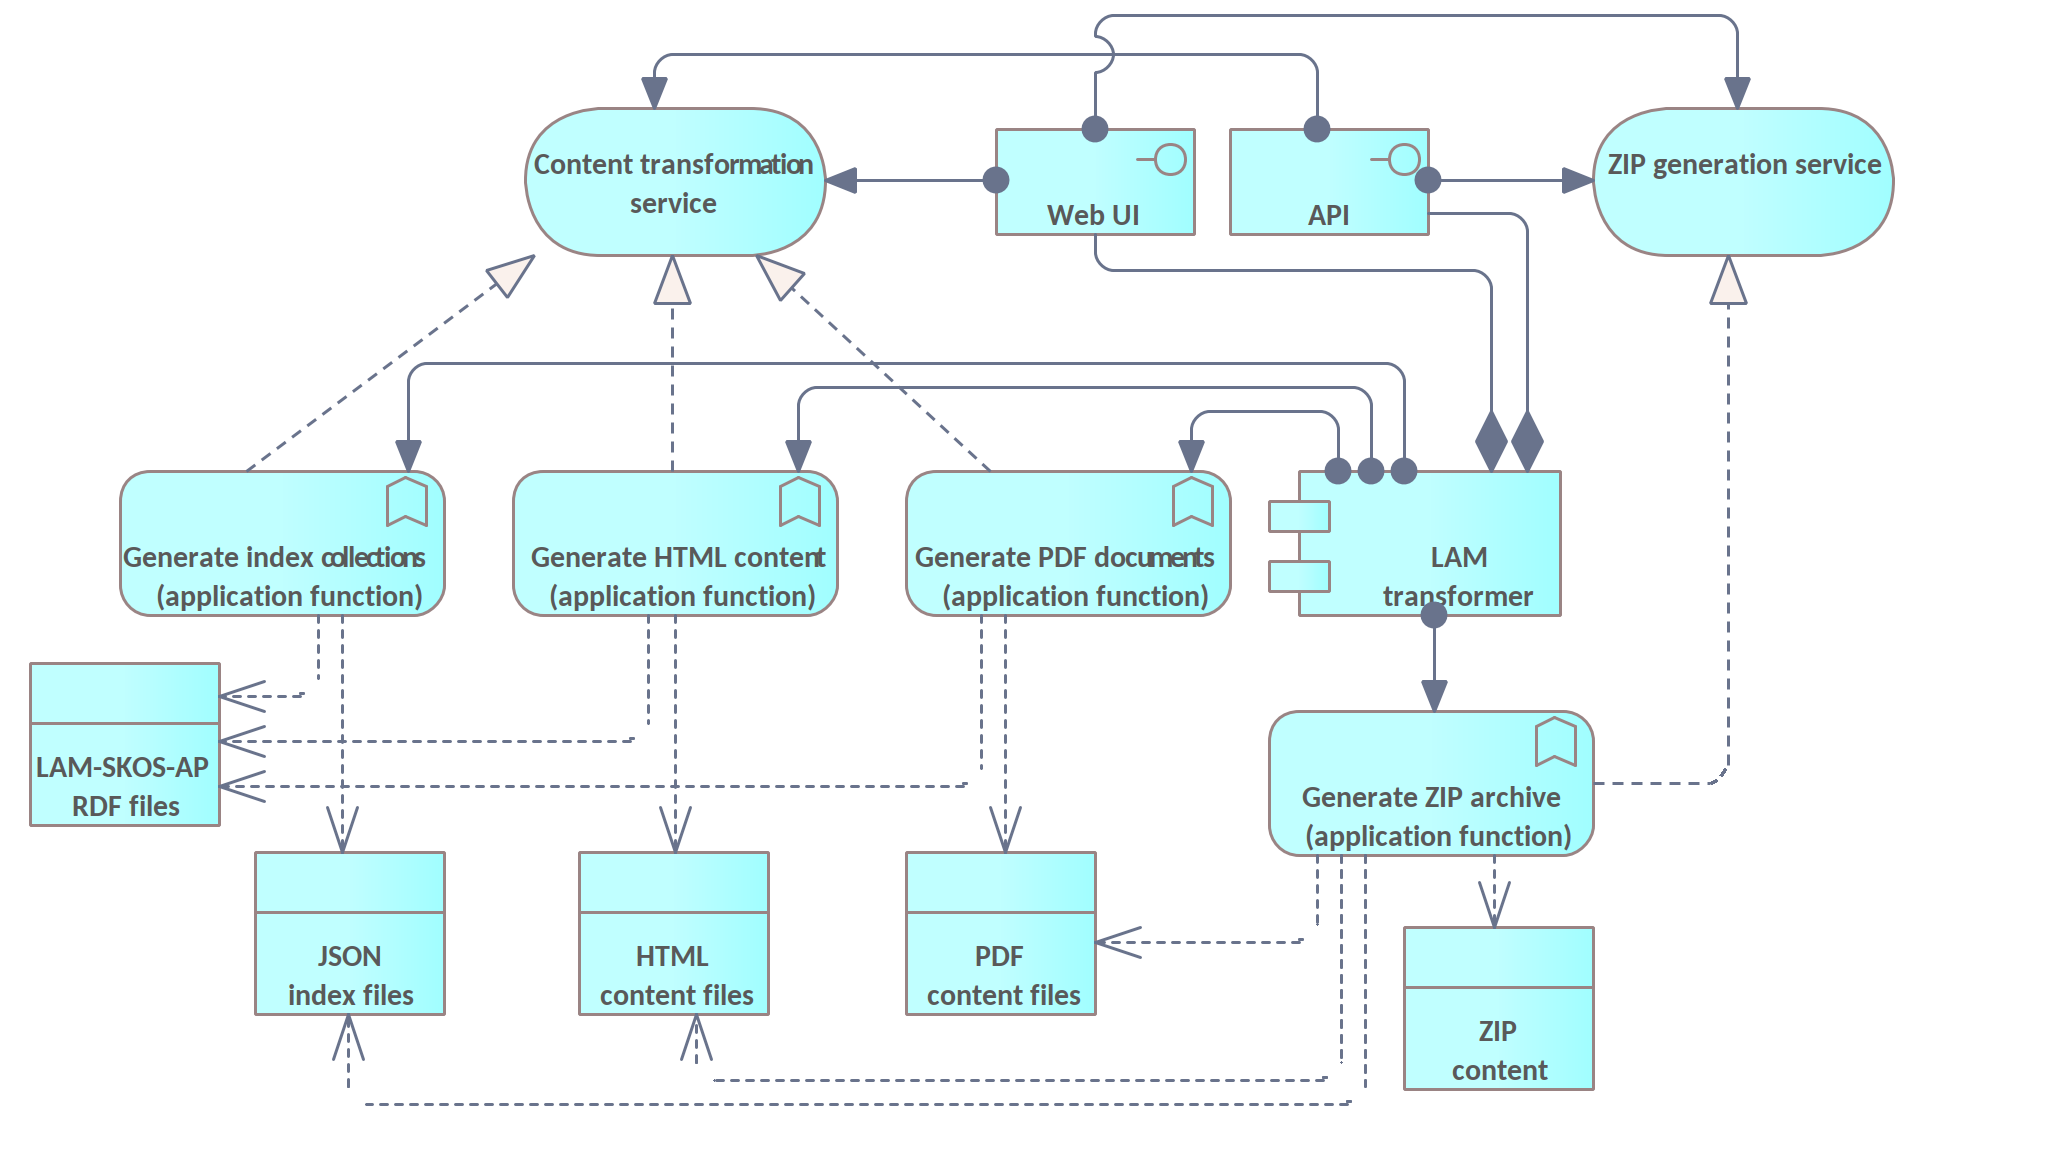
\includegraphics[width=.98\textwidth]{images/application/Content transformer.png}
		\caption{LAM transformation tool application architecture}
		\label{fig:app-transformation-tool}
	\end{figure}

	The main service this application exposes is the content transformation, positioned on the top of the diagram. This service is exposed through two interfaces: a web graphical user interface and an application programming interface. This service is realised by three application functionalities: generation of the HTML representation, generation of the PDF representation and generation of JSON indexes. The first two representations are meant to be distributed as such for the end-user consumption, while the indexes are meant to enable the search functionality provided by the OP Portal. The input taken by these functionalities shall be structured according to LAM-SKOS-AP\cite{lam-skos-ap-2019}.
	
	In order to facilitate the transmission of the artefacts generated by the LAM transformer, an additional service is foreseen, which aggregates the results of the transformation service into a ZIP archive. In the next section is described the LAM online tool, which ingests the ZIP archive and disseminates its content on a web interface. 
	
	\subsection{LAM online tool}
	
	The LAM online tool is a mini-website hosted within the OP Portal ecosystem. Its main services are the content import, content consultation and content search. Figure \ref{fig:app-online-tool-ingestion} depicts the architecture supporting the content ingestion. 
	
	
    \begin{figure}[!h]
		\centering
		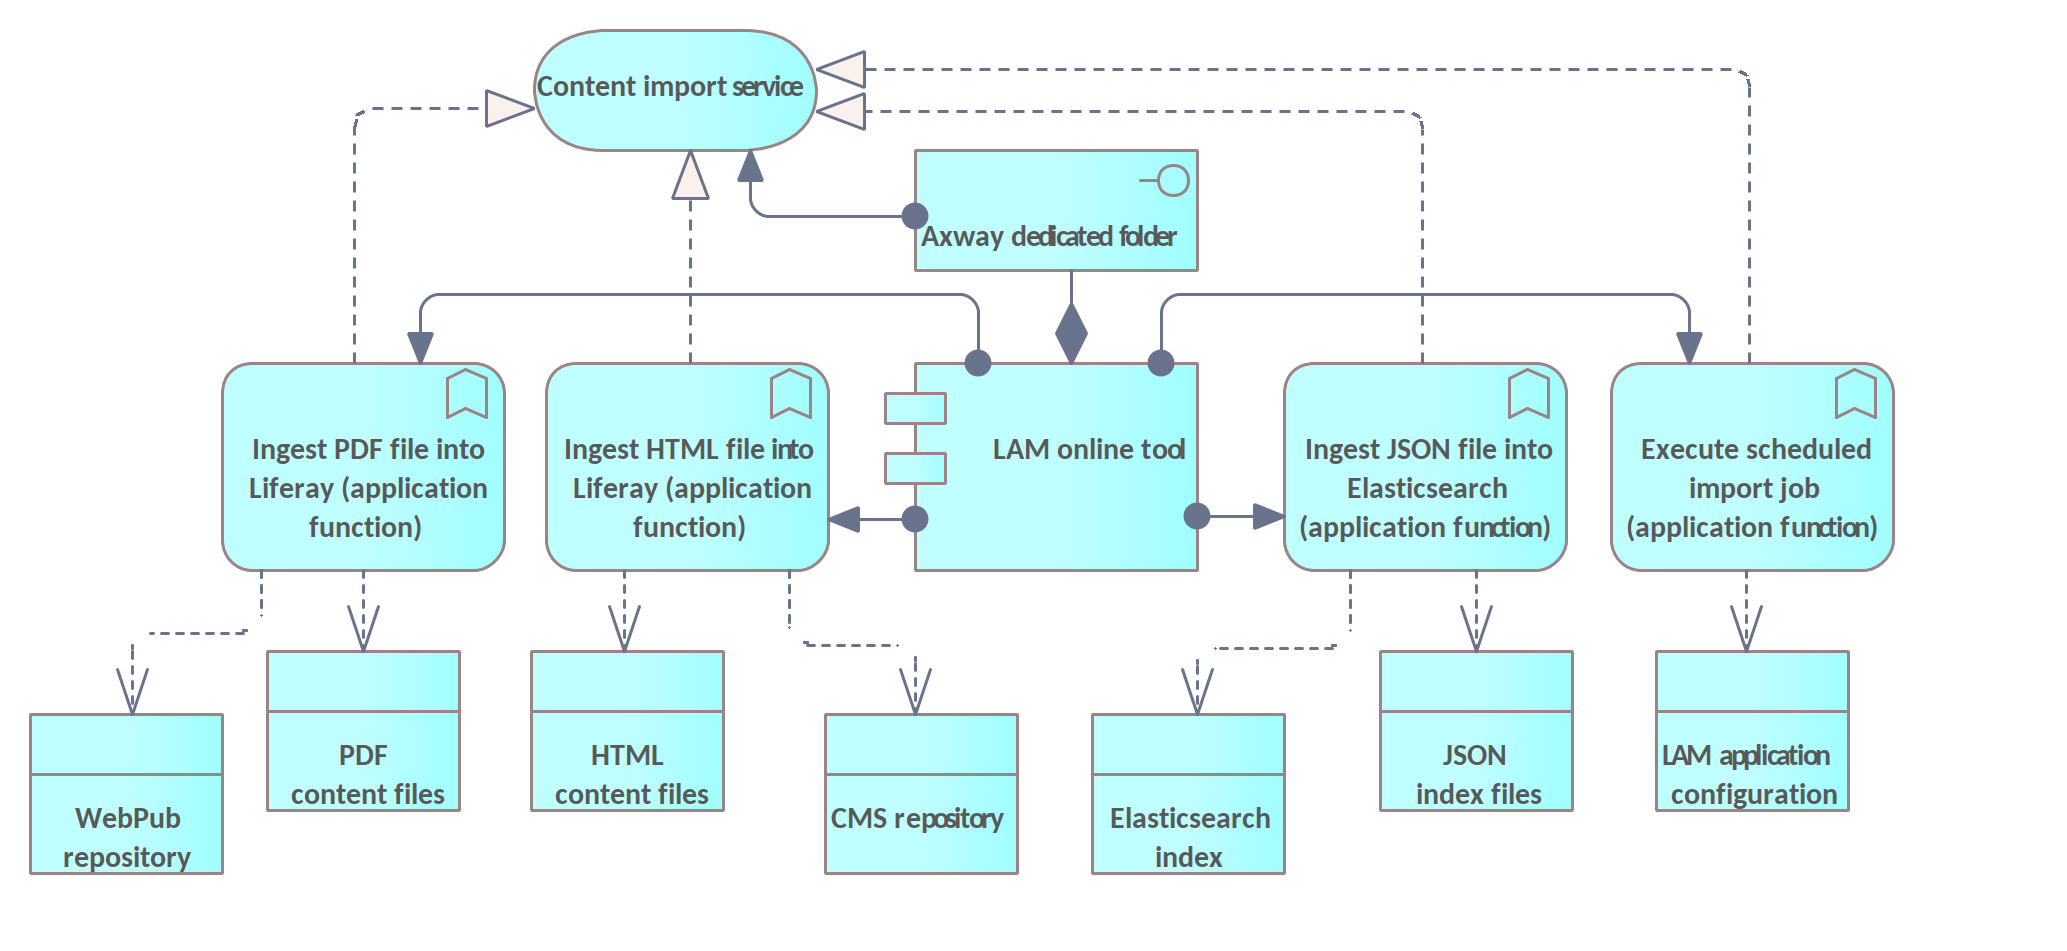
\includegraphics[width=.98\textwidth]{images/application/Online tool - import.png}
		\caption{LAM online tool application architecture: content import service}
		\label{fig:app-online-tool-ingestion}
	\end{figure}	

    \begin{figure}[!h]
	\centering
	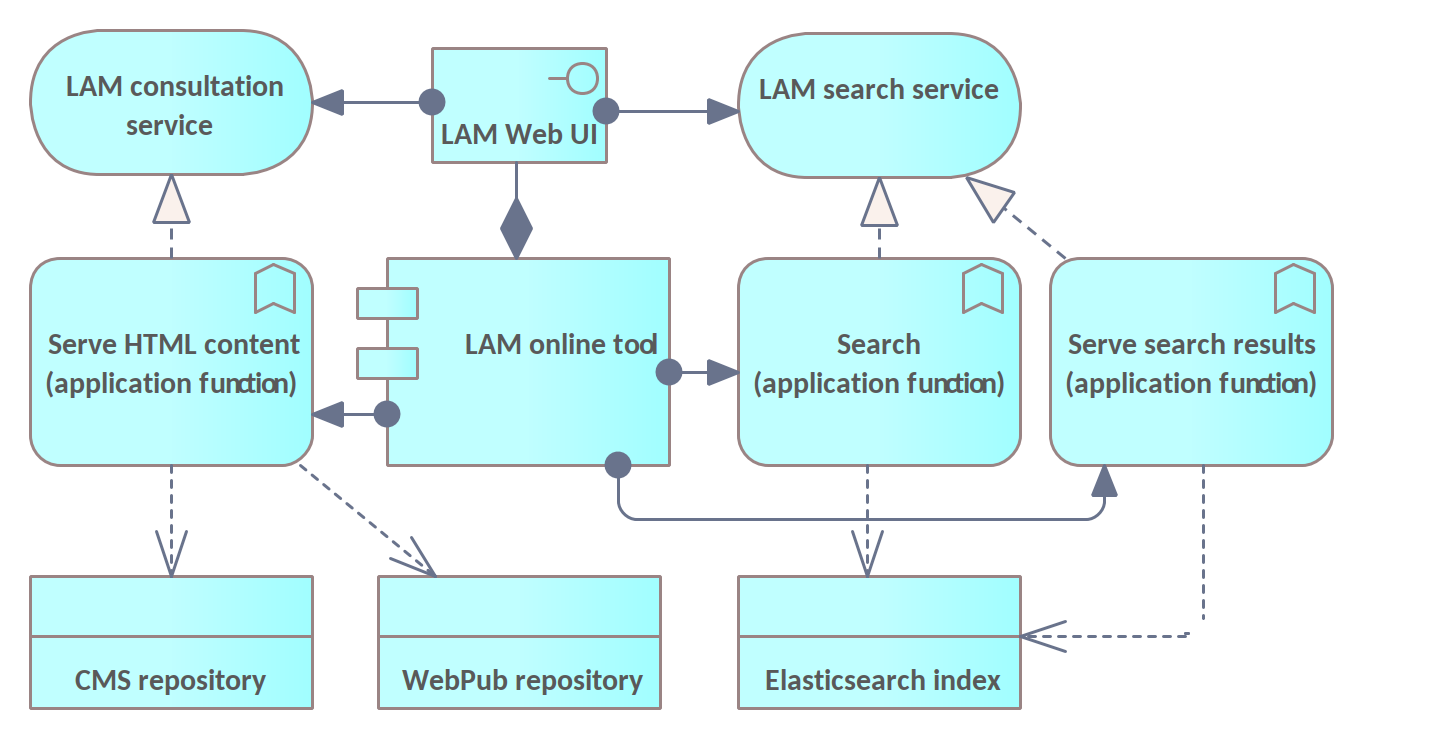
\includegraphics[width=.8\textwidth]{images/application/Online tool - dissemination.png}
	\caption{LAM online tool application architecture: content dissemination services}
	\label{fig:app-online-tool-dissemination}
	\end{figure}
	
	The import service is exposed through a dedicated Axway folder where a scheduled job regularly checks for new content. As soon as new content is placed there the ingestion functionality starts. The expected input is the ZIP archive containing the PDF, HTML and JSON content. When this archive is unpacked each of these representations is treated accordingly for different purposes.
	
	
	

    \begin{figure}[!h]
	\centering
	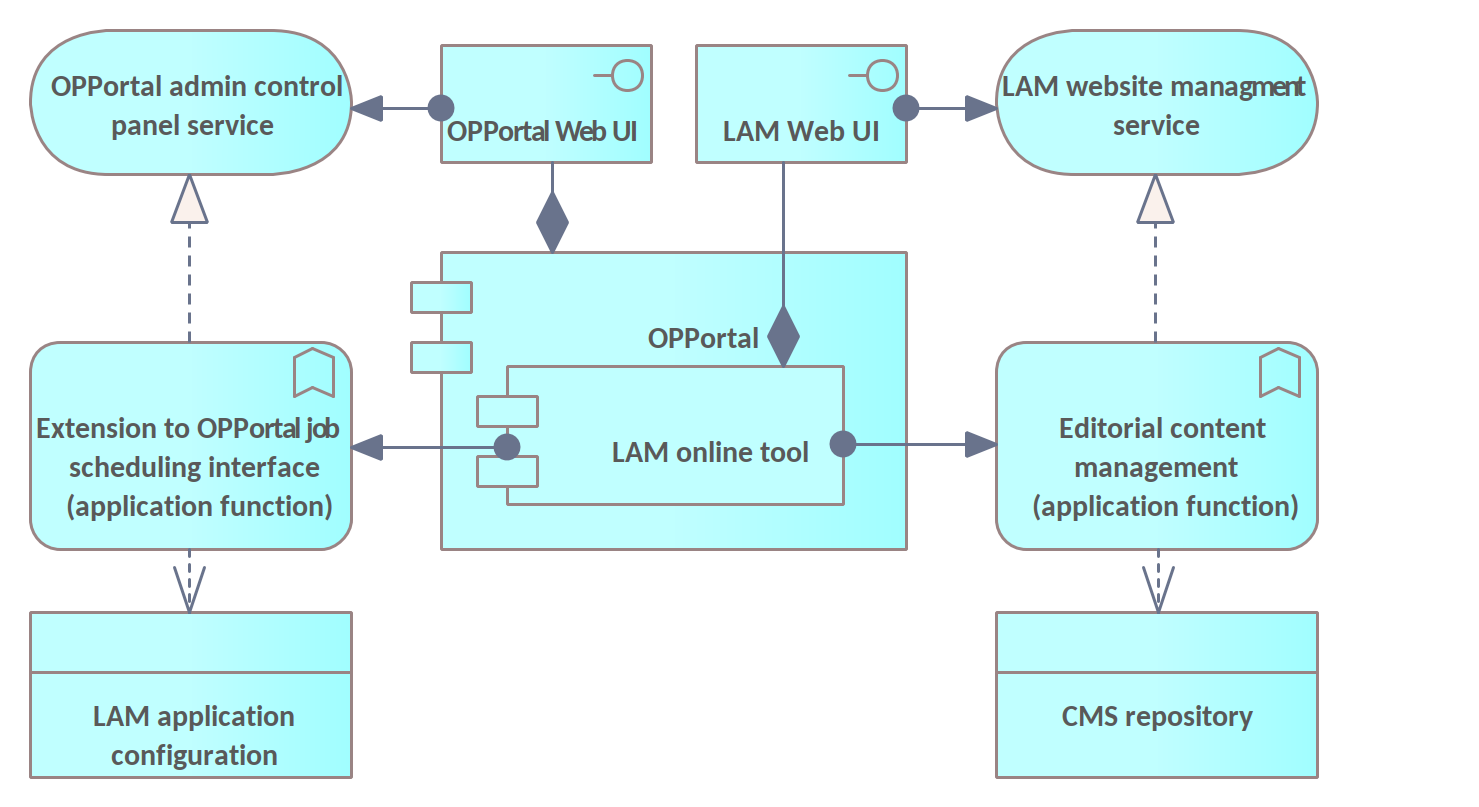
\includegraphics[width=.7\textwidth]{images/application/Online tool - management.png}
	\caption{LAM online tool application architecture: management services}
	\label{fig:app-online-tool-management}
	\end{figure}
	
	\subsection{LAM validation tool}

	\section{LAM lifecycle application architecture}
	\label{sec:application-lifecycle}
	
	\subsection{Evolution management}

    \begin{figure}[!h]
		\centering
		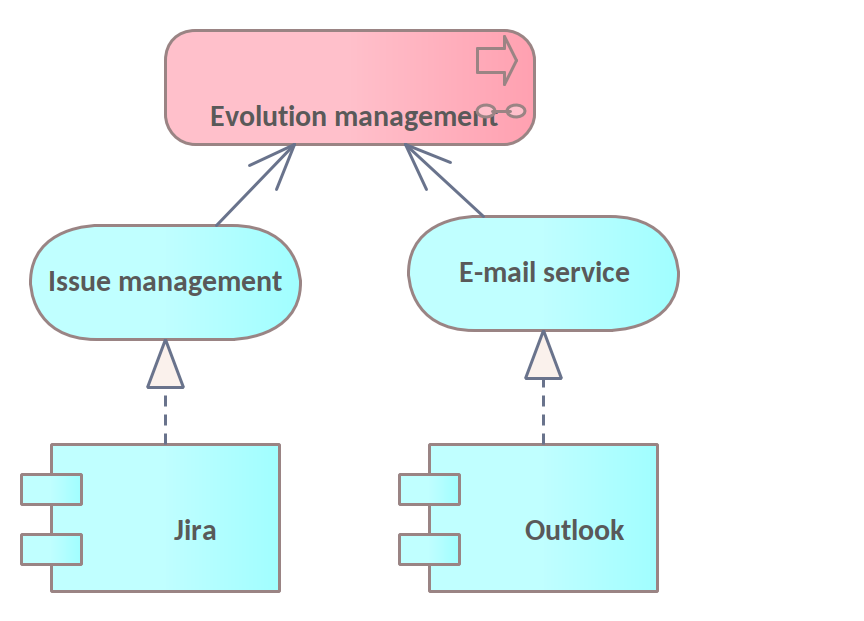
\includegraphics[width=.5\textwidth]{images/application/lifecycle/Evolution.png}
		\caption{Application services and component that serve evolution management lifecycle stage}
		\label{fig:app-evolution-management}
	\end{figure}
	
	\subsection{Implementation}
	
    \begin{figure}[!h]
		\centering
		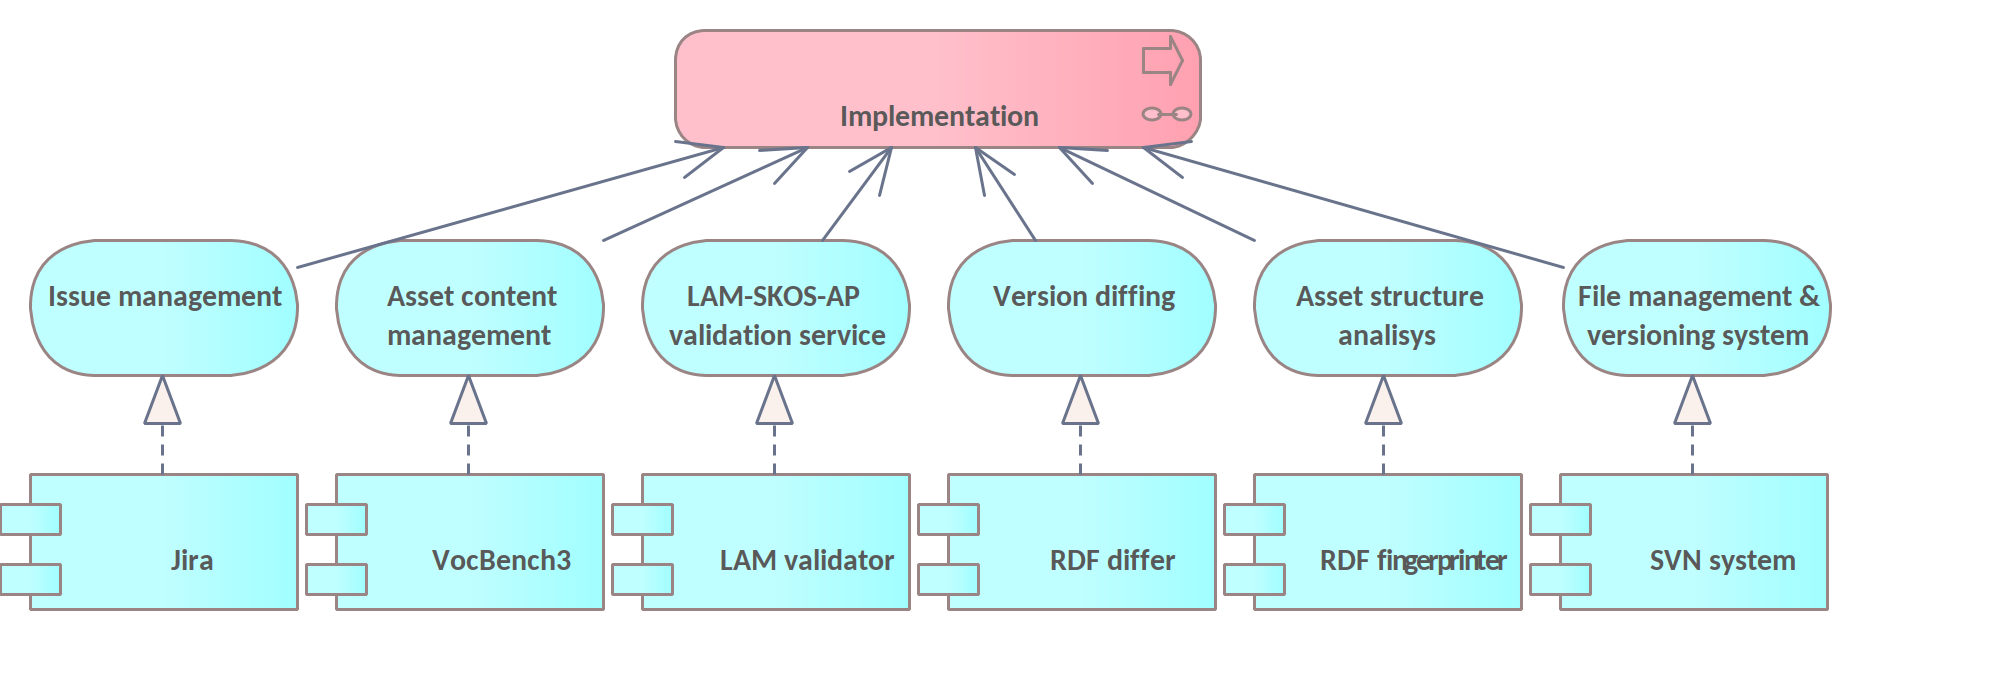
\includegraphics[width=.95\textwidth]{images/application/lifecycle/Implementation.png}
		\caption{Application services and component that serve implementation lifecycle stage}
		\label{fig:app-implementation}
	\end{figure}

	\subsection{Validation}

	 \begin{figure}[!h]
		\centering
		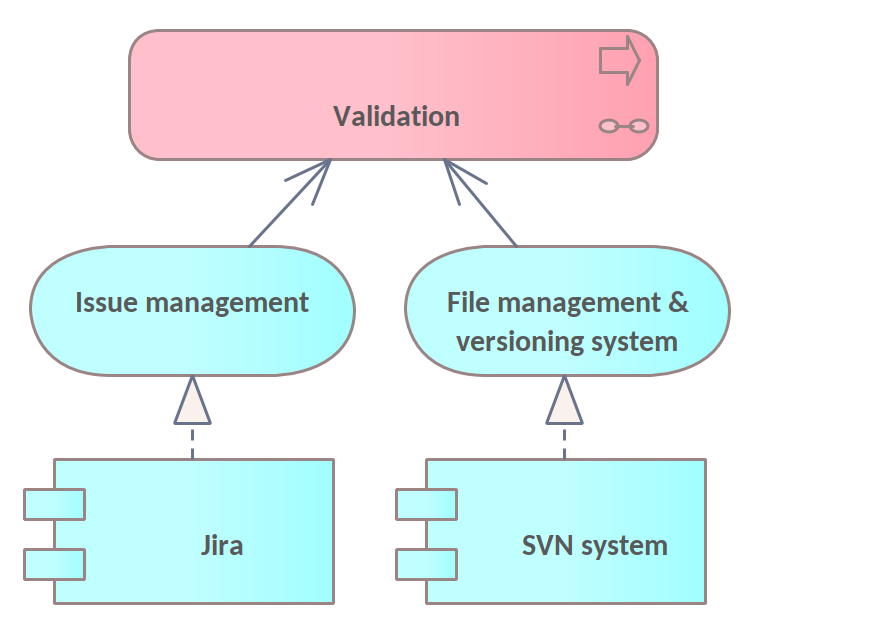
\includegraphics[width=.5\textwidth]{images/application/lifecycle/Validation.png}
		\caption{Application services and component that serve validation lifecycle stage}
		\label{fig:app-validation}
	\end{figure}	
	
	\subsection{Release}
	
	 \begin{figure}[!h]
		\centering
		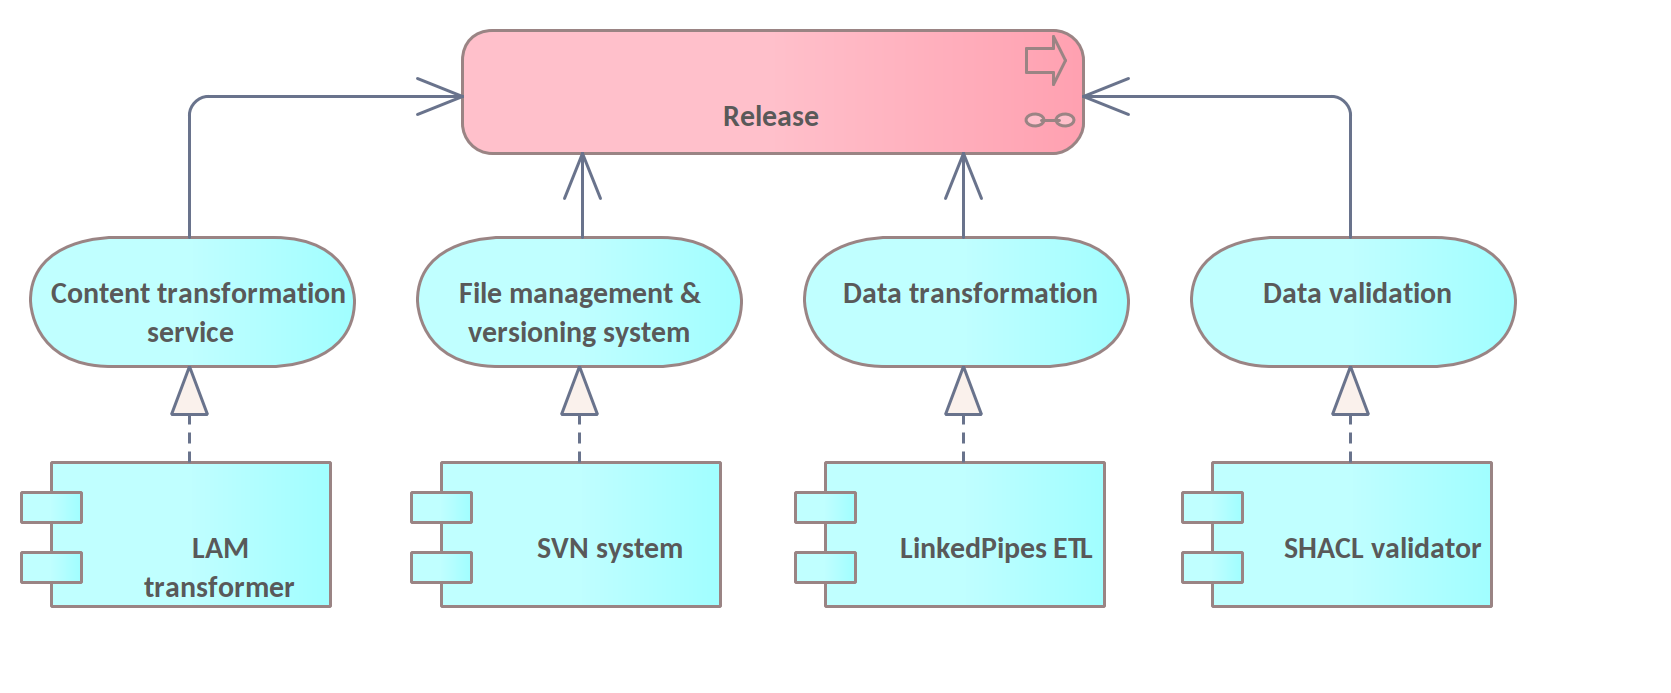
\includegraphics[width=.8\textwidth]{images/application/lifecycle/Release.png}
		\caption{Application services and component that serve release lifecycle stage}
		\label{fig:app-release}
	\end{figure}
	
	\subsection{Publication}
	
	 \begin{figure}[!h]
		\centering
		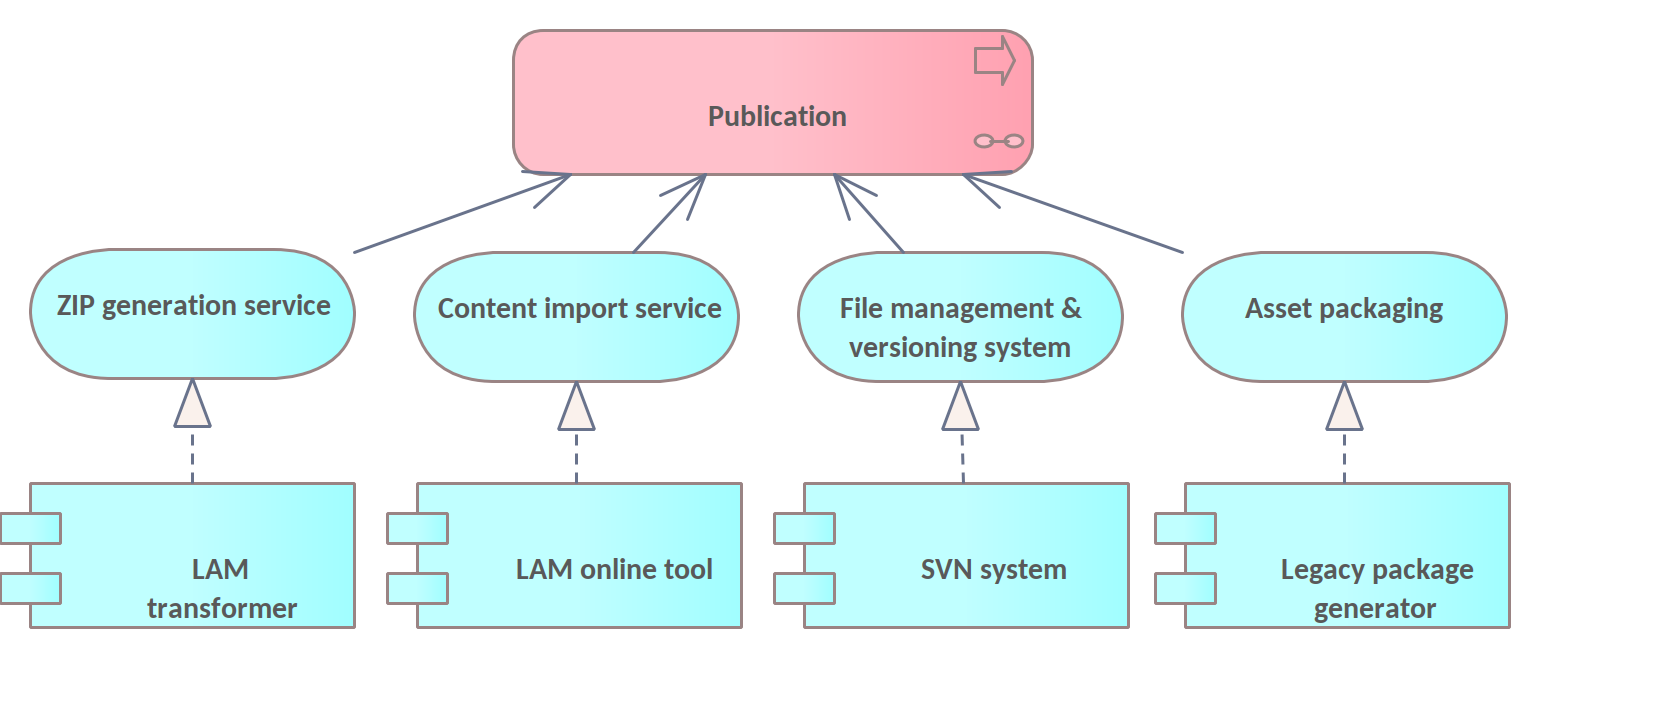
\includegraphics[width=.8\textwidth]{images/application/lifecycle/Publication.png}
		\caption{Application services and component that serve publication lifecycle stage}
		\label{fig:app-publication}
	\end{figure}